\documentclass{beamer}
% Use DS9 global theme (includes pgfplots for visualization)
\usepackage{../../../shared/templates/ds9_theme}
\graphicspath{{../images/}{../../../shared/images/}}

% Title page configuration
\title[Circular and Rotational Motion]{PHYS11 CH:6.1-6.2}
\subtitle{Circular \& Rotational Motion}
\author[Mr. Gullo]{Mr. Gullo}
\date[Oct 2024]{October 2024}

\begin{document}

\frame{\titlepage}

\begin{frame}
\frametitle{Learning Objectives}
By the end of this lesson, you will be able to:
\pause
\begin{itemize}
    \item Calculate angle of rotation ($\Delta\theta$) in radians given arc length and radius
    \pause
    \item Determine angular velocity ($\omega$) from rotational motion data
    \pause
    \item Apply the relationship between tangential velocity and angular velocity
    \pause
    \item Calculate centripetal acceleration for objects in circular motion
    \pause
    \item Determine the centripetal force required to maintain circular motion
    \pause
    \item Solve multi-step problems involving uniform circular motion
\end{itemize}
\end{frame}

\section{Key Concepts and Definitions}

\begin{frame}
\frametitle{Key Terms: Rotational Quantities}
\pause
\textbf{Angle of Rotation} ($\Delta \theta$):
\begin{itemize}
    \item Angular displacement
    \item Measured in radians (rad)
    \item One complete circle = $2\pi$ rad = 360°
\end{itemize}
\pause

\textbf{Arc Length} ($\Delta s$):
\begin{itemize}
    \item Distance traveled along circular path
    \item Related to angle and radius
\end{itemize}
\pause

\textbf{Radius of Curvature} ($r$):
\begin{itemize}
    \item Distance from center to object
    \item Determines size of circular path
\end{itemize}
\end{frame}

\begin{frame}
\frametitle{Visualizing Rotational Motion}
\textbf{Understanding the relationship between arc length, angle, and radius:}
\pause
\begin{itemize}
    \item An object moves along a circular path
    \pause
    \item The arc length ($\Delta s$) is the distance it travels
    \pause
    \item The angle ($\Delta\theta$) measures how far it rotates
    \pause
    \item The radius ($r$) determines the size of the circle
\end{itemize}
\end{frame}

\begin{frame}
\frametitle{Rotational Motion Diagram}
\pause
\begin{figure}[H]
    \centering
    \includegraphics[width=1\linewidth]{Screenshot 2024-11-21 125544.png}
    \caption{Arc length, angle, and radius relationship}
\end{figure}
\end{frame}

\begin{frame}
\frametitle{Key Terms: Angular Velocity}
\pause
\textbf{Angular Velocity} ($\omega$):
\begin{itemize}
    \item Rate of change of angle with time
    \pause
    \item Units: radians per second (rad/s)
    \pause
    \item Can also be expressed in revolutions per minute (rpm)
    \pause
    \item Describes how fast something rotates
\end{itemize}
\end{frame}

\begin{frame}
\frametitle{Understanding Angular Velocity}
\textbf{Before we see the equation:}
\pause
\begin{itemize}
    \item Angular velocity tells us rotation speed
    \pause
    \item Similar to linear velocity, but for rotation
    \pause
    \item Larger $\omega$ means faster spinning
\end{itemize}
\end{frame}

\begin{frame}
\frametitle{Angular Velocity Visualization}
\pause
\begin{figure}[H]
    \centering
    \includegraphics[width=0.6\linewidth]{Screenshot 2024-11-21 125846.png}
    \caption{Angular velocity definition}
\end{figure}
\end{frame}

\begin{frame}
\frametitle{Linear vs Angular Velocity}
\pause
\begin{figure}
    \centering
    \includegraphics[width=0.65\linewidth]{Screenshot 2024-11-21 132156.png}
    \caption{Connection between linear and angular motion}
\end{figure}
\end{frame}

\begin{frame}
\frametitle{Key Terms: Centripetal Quantities}
\pause
\textbf{Centripetal Acceleration} ($a_c$):
\begin{itemize}
    \item Acceleration directed toward center of circle
    \pause
    \item Changes velocity direction, not speed
    \pause
    \item Always perpendicular to velocity
\end{itemize}
\pause

\textbf{Centripetal Force} ($F_c$):
\begin{itemize}
    \item Net force causing circular motion
    \pause
    \item Points toward center of circle
    \pause
    \item Without it, object moves in straight line
\end{itemize}
\end{frame}

\begin{frame}
\frametitle{Understanding Centripetal Force}
\textbf{Key concept:}
\pause
\begin{itemize}
    \item Objects naturally move in straight lines (Newton's 1st Law)
    \pause
    \item To move in a circle requires constant inward force
    \pause
    \item This inward force is the centripetal force
    \pause
    \item Examples: tension in string, friction on tires, gravity
\end{itemize}
\end{frame}

\begin{frame}
\frametitle{Centripetal Force Visualization}
\pause
\begin{figure}
    \centering
    \includegraphics[width=0.5\linewidth]{Screenshot 2024-11-21 130344.png}
    \caption{Centripetal acceleration and force directions}
\end{figure}
\end{frame}

\section{Misconceptions}

\begin{frame}
\frametitle{The Fictitious Centrifugal Force}

\begin{columns}[T]
\begin{column}{0.6\textwidth}
\textbf{What is centrifugal "force"?}
\pause
\begin{itemize}
    \item Not a real force!
    \pause
    \item Appears in rotating reference frames
    \pause
    \item Feels like being "thrown outward"
\end{itemize}

\pause
\textbf{Examples in daily life:}
\begin{itemize}
    \item Car turning corner
    \pause
    \item Tea leaves gathering in cup center
    \pause
    \item Clothes in washing machine
\end{itemize}
\end{column}

\begin{column}{0.4\textwidth}
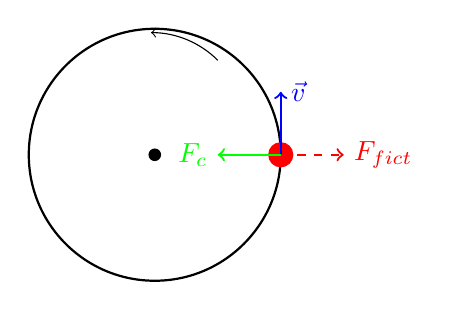
\begin{tikzpicture}[scale=0.8]
    \draw[thick] (0,0) circle (2cm);
    \fill[red] (2,0) circle (0.2cm);
    \draw[->,thick,blue] (2,0) -- (2,1) node[right] {$\vec{v}$};
    \draw[->,thick,red,dashed] (2,0) -- (3,0) node[right] {$F_{fict}$};
    \draw[->,thick,green] (2,0) -- (1,0) node[left] {$F_c$};
    \fill (0,0) circle (0.1cm);
    \draw[->] (1,1.5) arc (45:90:1.5cm);
\end{tikzpicture}
\end{column}
\end{columns}
\end{frame}

\begin{frame}
\frametitle{Why Centrifugal Force Isn't Real}
\textbf{Remember:}
\pause
\begin{itemize}
    \item Objects want straight-line motion (inertia)
    \pause
    \item What feels like "outward force" is your body resisting direction change
    \pause
    \item Real force is centripetal (inward), causing circular path
    \pause
    \item No outward force actually exists in inertial reference frame
\end{itemize}
\pause

\vspace{0.5cm}
\small{\url{https://en.wikipedia.org/wiki/Centrifugal_force}}
\end{frame}

\section{Essential Equations}

\begin{frame}
\frametitle{Important Equations}
\pause
\begin{align*}
\text{Angle of Rotation:} & \quad \Delta \theta = \frac{\Delta s}{r} \quad \text{(rad)} \\[0.8em]
\pause
\text{Angular Velocity:} & \quad \omega = \frac{\Delta \theta}{\Delta t} \quad \text{(rad/s)} \\[0.8em]
\pause
\text{Tangential Velocity:} & \quad v = r\omega \quad \text{(m/s)} \\[0.8em]
\pause
\text{Centripetal Acceleration:} & \quad a_c = \frac{v^2}{r} = r\omega^2 \quad \text{(m/s}^2\text{)} \\[0.8em]
\pause
\text{Centripetal Force:} & \quad F_c = \frac{mv^2}{r} = mr\omega^2 \quad \text{(N)}
\end{align*}
\end{frame}

\section{I Do Example}

\begin{frame}
\frametitle{I Do: Problem Statement}
\pause
\textbf{Problem:}

A car drives around a circular track of radius 100 m at constant speed of 20 m/s.
\pause
\begin{enumerate}
    \item Calculate the centripetal acceleration
    \item Find the centripetal force if car mass is 1500 kg
\end{enumerate}
\end{frame}

\begin{frame}
\frametitle{I Do: Part 1 - G and U}
\pause
\begin{columns}[T]
\column{0.48\textwidth}
\textbf{G - Givens}
\begin{itemize}
    \item $r = 100$ m
    \item $v = 20$ m/s
    \item $m = 1500$ kg
\end{itemize}

\column{0.48\textwidth}
\textbf{U - Unknown}
\begin{itemize}
    \item Part 1: $a_c = ?$
    \item Part 2: $F_c = ?$
\end{itemize}
\end{columns}
\end{frame}

\begin{frame}
\frametitle{I Do: Part 1 - E}
\pause
\textbf{E - Equation}
\begin{itemize}
    \item Need centripetal acceleration
    \pause
    \item Use: $a_c = \frac{v^2}{r}$
    \pause
    \item Already solved for $a_c$
\end{itemize}
\end{frame}

\begin{frame}
\frametitle{I Do: Part 1 - S and S}
\pause
\textbf{S - Substitute}
\begin{itemize}
    \item $a_c = \frac{(20 \text{ m/s})^2}{100 \text{ m}}$
\end{itemize}
\pause

\textbf{S - Solve}
\begin{itemize}
    \item $a_c = \frac{400 \text{ m}^2\text{/s}^2}{100 \text{ m}}$
    \pause
    \item $a_c = 4$ m/s$^2$
    \pause
    \item \boxed{a_c = 4 \text{ m/s}^2}
\end{itemize}
\end{frame}

\begin{frame}
\frametitle{I Do: Part 2 - E}
\pause
\textbf{E - Equation}
\begin{itemize}
    \item Need centripetal force
    \pause
    \item Use: $F_c = ma_c$
    \pause
    \item Already solved for $F_c$
\end{itemize}
\end{frame}

\begin{frame}
\frametitle{I Do: Part 2 - S and S}
\pause
\textbf{S - Substitute}
\begin{itemize}
    \item $F_c = (1500 \text{ kg})(4 \text{ m/s}^2)$
\end{itemize}
\pause

\textbf{S - Solve}
\begin{itemize}
    \item $F_c = 6000$ kg·m/s$^2$
    \pause
    \item $F_c = 6000$ N
    \pause
    \item \boxed{F_c = 6000 \text{ N}}
\end{itemize}
\end{frame}

\section{We Do Example}

\begin{frame}
\frametitle{We Do: Problem Statement}
\pause
\textbf{Let's solve together:}

A CD spins at 300 rpm (revolutions per minute).
\pause
\begin{enumerate}
    \item Convert rpm to angular velocity in rad/s
    \item Calculate tangential velocity at $r = 6$ cm
\end{enumerate}
\end{frame}

\begin{frame}
\frametitle{We Do: Part 1 Setup}
\textbf{What do we know?}
\pause
\begin{itemize}
    \item Given: 300 rpm
    \pause
    \item Unknown: $\omega$ in rad/s
    \pause
    \item Need conversion factors
\end{itemize}
\pause

\textbf{Conversion factors needed:}
\begin{itemize}
    \item 1 revolution = $2\pi$ radians
    \item 1 minute = 60 seconds
\end{itemize}
\end{frame}

\begin{frame}
\frametitle{We Do: Part 1 Solution}
\textbf{Your turn: Set up conversion}
\pause

\[ \omega = 300 \frac{\text{rev}}{\text{min}} \times \frac{2\pi \text{ rad}}{1 \text{ rev}} \times \frac{1 \text{ min}}{60 \text{ s}} \]
\pause

\textbf{Calculate:}
\[ \omega = \frac{300 \times 2\pi}{60} = 31.4 \text{ rad/s} \]
\pause

\[\boxed{\omega = 31.4 \text{ rad/s}}\]
\end{frame}

\begin{frame}
\frametitle{We Do: Part 2 Setup}
\pause
\textbf{Now find tangential velocity:}
\begin{itemize}
    \item Given: $r = 6$ cm $= 0.06$ m, $\omega = 31.4$ rad/s
    \pause
    \item Unknown: $v = ?$
    \pause
    \item Equation: $v = r\omega$
\end{itemize}
\pause

\textbf{Your turn: Calculate}
\end{frame}

\begin{frame}
\frametitle{We Do: Part 2 Solution}
\pause
\textbf{Substitute and solve:}
\pause

\[ v = r\omega = (0.06 \text{ m})(31.4 \text{ rad/s}) \]
\pause

\[ v = 1.88 \text{ m/s} \]
\pause

\[\boxed{v = 1.88 \text{ m/s}}\]
\end{frame}

\section{You Do Example}

\begin{frame}
\frametitle{You Do: Practice Problem}
\pause
\textbf{Solve independently:}

A ball attached to string is swung in horizontal circle with radius 0.5 m. Ball makes one complete revolution in 1.2 seconds.

\pause
\textbf{Find:}
\begin{enumerate}
    \item Angular velocity
    \item Centripetal acceleration
    \item Tension in string if ball mass is 0.2 kg
\end{enumerate}

\pause
\vspace{0.5cm}
\textbf{Hint:} Use GUESS method. Start with what you know!
\end{frame}

\section{Summary}

\begin{frame}
\frametitle{Summary}
\textbf{Key takeaways:}
\pause
\begin{itemize}
    \item Circular motion requires centripetal force directed toward center
    \pause
    \item $a_c$ and $F_c$ always point inward, never outward
    \pause
    \item Angular quantities ($\theta$, $\omega$) convert to linear ($s$, $v$) using radius
    \pause
    \item Uniform circular motion: constant speed, changing velocity direction
    \pause
    \item Centrifugal "force" is not real - it's inertia resisting direction change
    \pause
    \item Use GUESS method for systematic problem solving
\end{itemize}
\end{frame}

\end{document}